\documentclass[usenames,dvipsnames,svgnames,table,aspectratio=169]{beamer}

\usepackage[utf8]{inputenc}
\usepackage{soul}
\usepackage{listings}
\usepackage{tikz}
\usepackage{booktabs}
\usepackage{minted}
\usepackage{biblatex}

\usetheme{laas}

\AtBeginSection[]{
  \begin{frame}
  \vfill
  \centering
  \begin{beamercolorbox}[sep=8pt,center,shadow=true,rounded=true]{title}
    \usebeamerfont{title}\insertsectionhead\par%
  \end{beamercolorbox}
  \vfill
  \end{frame}
}

\lstset{language=C++,
                basicstyle=\ttfamily,
                keywordstyle=\color{blue}\ttfamily,
                stringstyle=\color{red}\ttfamily,
                commentstyle=\color{purple}\ttfamily,
                morecomment=[l][\color{magenta}]{\#}
}


\title{Modern C++ Best Practices}
\author{Tim Luchterhand, based on a presentation by Paul Nykiel \cite{Nykiel2020}}
\date{\today}

\addbibresource{bibliography.bib}
\begin{document}
\maketitle

\frame{
    \tableofcontents
}

\section{Introduction}
\begin{frame}
    \frametitle{Features of C++}
    \begin{itemize}
        \item<+-> C++ $\neq$ C with classes!
        \item<+-> Deterministic lifetime of objects
        \item<+-> No garbage collection
        \item<+-> Undefined behavior
    \end{itemize}
\end{frame}

\begin{frame}
    \frametitle{Goals of this Talk}
    \begin{itemize}
        \item<+-> Avoid undefined behavior at all times
        \item<+-> Let go of old habits from C, do not use C constructs if not necessary
        \begin{itemize}
            \item<+-> C-Arrays
            \item<+-> Pointers
            \item<+-> Manual memory management
        \end{itemize}
        \item<+-> Focus on logic instead of low level data structures and memory management
        \item<+-> Use the stl
    \end{itemize}
\end{frame}

\section{Memory Layout}
\begin{frame}
    \frametitle{Stack and Heap}
    \begin{columns}
        \begin{column}{.5\textwidth}
            \begin{itemize}
                \item<+-> System memory (RAM) is divided in two parts
                \item<+-> Stack is used for function calls
                \item<+-> Heap is used for dynamically allocated memory
                \item<+-> Allocated memory on the heap needs to be freed \textit{manually}
                \item<+-> If there is more than one owner this can get complicated
            \end{itemize}
        \end{column}
        \begin{column}{.5\textwidth}
            \begin{figure}[H]
                \centering
                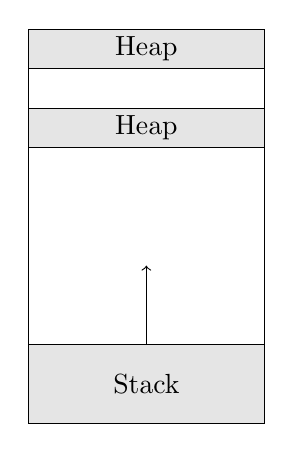
\begin{tikzpicture}
                    \draw [draw] (0,0) rectangle (3,5);
                    \filldraw [draw=black,fill=gray!20] (0,0) rectangle (3,1) node[pos=.5] {Stack};
                    \filldraw [draw=black,fill=gray!20] (0,4.5) rectangle (3,5) node[pos=.5] {Heap};
                    \filldraw [draw=black,fill=gray!20] (0,3.5) rectangle (3,4) node[pos=.5] {Heap};
                    \draw [->] (1.5,1) -- (1.5,2);
                \end{tikzpicture}
            \end{figure}
        \end{column}
    \end{columns}
\end{frame}

\begin{frame}
    \frametitle{Example: Stack}
    \begin{columns}
        \begin{column}{.5\textwidth}
            \lstinputlisting{examples/slides/stack.c}
        \end{column}
        \begin{column}{.5\textwidth}
            \begin{figure}[H]
                \centering
                \only<1> {
                    \begin{tikzpicture}
                        \draw [draw] (0,0) rectangle (3,6);
                    \end{tikzpicture}
                }
                \only<2,6> {
                    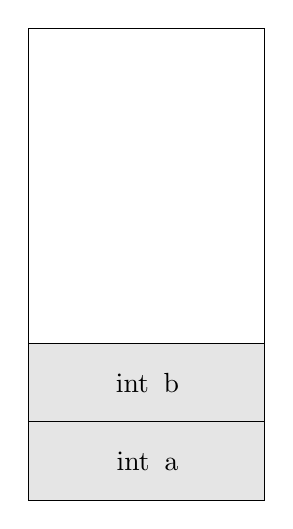
\begin{tikzpicture}
                        \draw [draw] (0,0) rectangle (3,6);
                        \filldraw [draw=black,fill=gray!20] (0,0) rectangle (3,1) node[pos=.5] {\lstinline{int a}};
                        \filldraw [draw=black,fill=gray!20] (0,1) rectangle (3,2) node[pos=.5] {\lstinline{int b}};
                    \end{tikzpicture}
                }
                \only<3> {
                    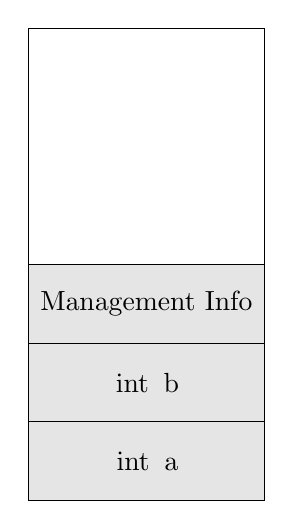
\begin{tikzpicture}
                        \draw [draw] (0,0) rectangle (3,6);
                        \filldraw [draw=black,fill=gray!20] (0,0) rectangle (3,1) node[pos=.5] {\lstinline{int a}};
                        \filldraw [draw=black,fill=gray!20] (0,1) rectangle (3,2) node[pos=.5] {\lstinline{int b}};
                        \filldraw [draw=black,fill=gray!20] (0,2) rectangle (3,3) node[pos=.5] {Management Info};
                    \end{tikzpicture}
                }
                \only<4> {
                    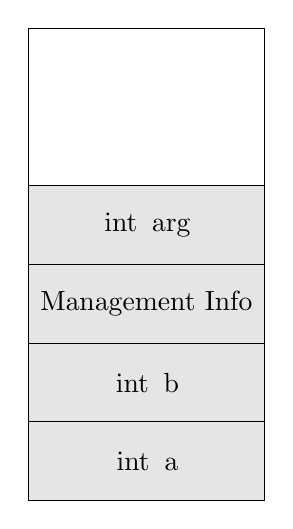
\begin{tikzpicture}
                        \draw [draw] (0,0) rectangle (3,6);
                        \filldraw [draw=black,fill=gray!20] (0,0) rectangle (3,1) node[pos=.5] {\lstinline{int a}};
                        \filldraw [draw=black,fill=gray!20] (0,1) rectangle (3,2) node[pos=.5] {\lstinline{int b}};
                        \filldraw [draw=black,fill=gray!20] (0,2) rectangle (3,3) node[pos=.5] {Management Info};
                        \filldraw [draw=black,fill=gray!20] (0,3) rectangle (3,4) node[pos=.5] {\lstinline{int arg}};
                    \end{tikzpicture}
                }
                \only<5> {
                    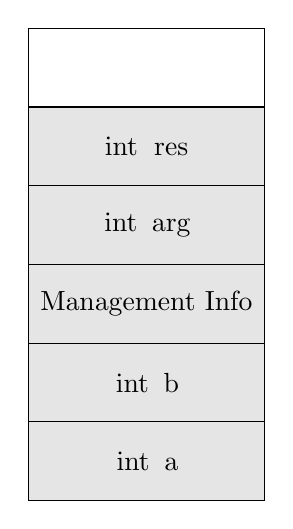
\begin{tikzpicture}
                        \draw [draw] (0,0) rectangle (3,6);
                        \filldraw [draw=black,fill=gray!20] (0,0) rectangle (3,1) node[pos=.5] {\lstinline{int a}};
                        \filldraw [draw=black,fill=gray!20] (0,1) rectangle (3,2) node[pos=.5] {\lstinline{int b}};
                        \filldraw [draw=black,fill=gray!20] (0,2) rectangle (3,3) node[pos=.5] {Management Info};
                        \filldraw [draw=black,fill=gray!20] (0,3) rectangle (3,4) node[pos=.5] {\lstinline{int arg}};
                        \filldraw [draw=black,fill=gray!20] (0,4) rectangle (3,5) node[pos=.5] {\lstinline{int res}};
                    \end{tikzpicture}
                }
            \end{figure}
        \end{column}
    \end{columns}
\end{frame}

\begin{frame}
    \Huge{Is that not enough?}
\end{frame}

\begin{frame}
    \frametitle{Example: Heap}
    \begin{columns}
        \begin{column}{.5\textwidth}
            \lstinputlisting{examples/slides/heap.cpp}
        \end{column}
        \begin{column}{.5\textwidth}
            \begin{figure}[H]
                \centering
                \only<1> {
                    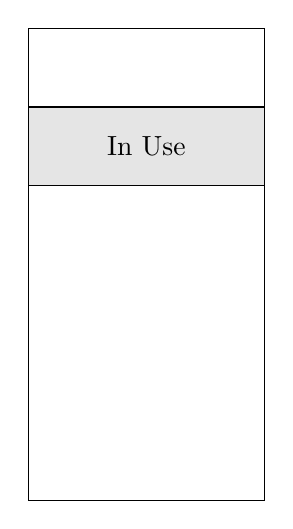
\begin{tikzpicture}
                        \draw [draw] (0,0) rectangle (3,6);
                        \filldraw [draw=black,fill=gray!20] (0,5) rectangle (3,4) node[pos=.5] {In Use};
                    \end{tikzpicture}
                }
                \only<2> {
                    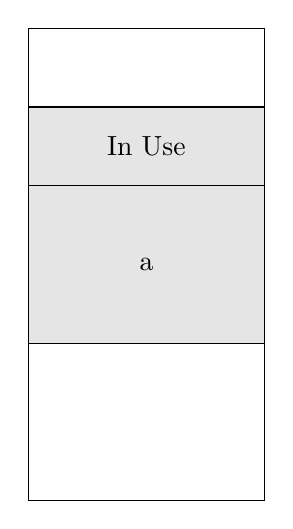
\begin{tikzpicture}
                        \draw [draw] (0,0) rectangle (3,6);
                        \filldraw [draw=black,fill=gray!20] (0,5) rectangle (3,4) node[pos=.5] {In Use};
                        \filldraw [draw=black,fill=gray!20] (0,4) rectangle (3,2) node[pos=.5] {\lstinline{a}};
                    \end{tikzpicture}
                }
                \only<3> {
                    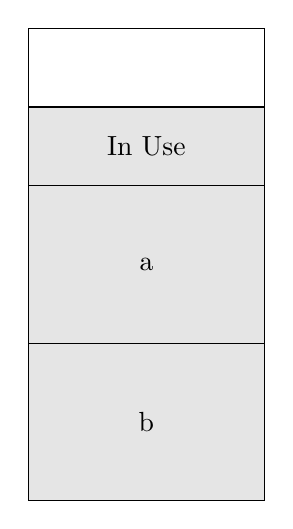
\begin{tikzpicture}
                        \draw [draw] (0,0) rectangle (3,6);
                        \filldraw [draw=black,fill=gray!20] (0,5) rectangle (3,4) node[pos=.5] {In Use};
                        \filldraw [draw=black,fill=gray!20] (0,4) rectangle (3,2) node[pos=.5] {\lstinline{a}};
                        \filldraw [draw=black,fill=gray!20] (0,2) rectangle (3,0) node[pos=.5] {\lstinline{b}};
                    \end{tikzpicture}
                }
                \only<4> {
                    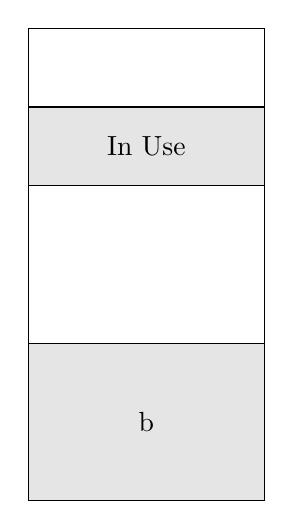
\begin{tikzpicture}
                        \draw [draw] (0,0) rectangle (3,6);
                        \filldraw [draw=black,fill=gray!20] (0,5) rectangle (3,4) node[pos=.5] {In Use};
                        \filldraw [draw=black,fill=gray!20] (0,2) rectangle (3,0) node[pos=.5] {\lstinline{b}};
                    \end{tikzpicture}
                }
            \end{figure}
        \end{column}
    \end{columns}
\end{frame}

\begin{frame}
    \frametitle{Object Lifetime}
    \lstinputlisting{examples/slides/lifetime.cpp}
\end{frame}

\begin{frame}
    \frametitle{Memory Leak}
    \lstinputlisting{examples/slides/memory_leak.cpp}
\end{frame}


\section{Zero Copy, Function Parameters and Aliases}
\begin{frame}
    \frametitle{C++ Copies by Default}
    \begin{itemize}
        \item<+-> \lstinputlisting{examples/slides/copy.cpp}
        \item<+-> \textit{Every} assignment is a copy
        \item<+-> Very simple
        \item<+-> Bad Performance for large objects
    \end{itemize}
\end{frame}

\begin{frame}
    \frametitle{References}
    \lstinputlisting{examples/slides/references.cpp}
\end{frame}

\begin{frame}
    \frametitle{Alias References}
    \lstinputlisting{examples/slides/references1.cpp}
\end{frame}

\begin{frame}
    \frametitle{Don't Overdo it}
    \lstinputlisting{examples/slides/references2.cpp}
\end{frame}

\begin{frame}
    \frametitle{Smart-Pointer}
    \begin{itemize}
        \item Standardlibrary kann Verwaltung übernehmen
            \pause
        \item \lstinline{unique\_ptr}
            \pause
        \item Genau ein Owner
            \pause
        \item
            \lstinline{std::unique\_ptr<int> a = std::make\_unique<int>(17);}
            \pause
        \item \lstinline{shared\_ptr}
            \pause
        \item Quasi immer nutzbar
            \pause
        \item
            \lstinline{std::shared\_ptr<int> a = std::make\_shared<int>(17);}
    \end{itemize}
\end{frame}

\begin{frame}
    \frametitle{Referenzen}
    \begin{itemize}
        \item Sprachfeature kein Library-Feature
            \pause
        \item Können nicht null sein
            \pause
        \item Können aber ungültig werden
            \pause
        \item
            \lstinline{int b = 17; int &a = b;}
    \end{itemize}
\end{frame}

\begin{frame}
    \frametitle{Zusammenfassung Pointer}
    \begin{itemize}
        \item Raw-Pointer: Sollten quasi nie verwendet werden
            \pause
        \item Unique-Pointer: Oftmals Ersatz für Raw-Pointer
            \pause
        \item Shared-Pointer: Sichere Pointer für beliebig viele Owner
            \pause
        \item Referenzen: Oftmals um Kopien zu vermeiden
    \end{itemize}
\end{frame}

\begin{frame}
    \Huge{Beispiel: Pointer \& Referenzen}
\end{frame}

\section*{References}
\begin{frame}
  \frametitle{References}
  \printbibliography
\end{frame}

\end{document}
